\section{Architecture Synthesis}

\subsection{General}

Goal: Determine a hardware architecture that efficiently executes a given algorithm.

\begin{itemize}[noitemsep]
\item Allocation: the necessary hardware resources
\item Scheduling: the timing of individual operations
\item Binding: the relation between individual operations of the algorithm and hardware resources
\end{itemize}

\subsection{Model}

\begin{itemize}[noitemsep]
\item $V_S$: the set of all operations.
\item Sequence Graph $G_s$ = ($V_S$,$E_S$).
\item $V_T$: the set of all resource types (eg. ALU, float-unit)
\item $V_R = V_S \cup V_T$
\item Resource graph $G_R$ = ($V_R$,$E_R$). Notice, the $G_R$ is bipartite and denotes, which operation can be executed by which resource.
\item $c: V_T \mapsto \mathbb{Z}$ (cost)
\item $w: E_R \mapsto \mathbb{Z}_{\geq(0)}$(execution time)
\end{itemize}

\subsection{Classification}

\begin{itemize}[noitemsep]
\item heuristics or exact methods
\item unlimited resources: no constraints in terms of the available resources are defined.
\item limited resources: constrains are given in terms of the number a types of available resources.
\item iterative algorithms: an initial solution to the architecture synthesis is improved step by step.
\item constructive algorithms: the synthesis problem is solved in one step.
\item transformative algorithms: the initial problem formulation is converted into a (classical) optimization problem
\end{itemize}

\subsection{Allocation, Binding, Scheduling, Latency, Mobility}

\begin{definition}[Allocation]
An allocation is a function $\alpha : V_T \rightarrow \mathbb{Z} \geq 0$ that assigns to each resource type $v_t \in V_T$ the number $\alpha(v_t)$ of available instances.
\end{definition}

\begin{definition}[Binding]
A binding is defined as a function $\beta: V_S \rightarrow V_T $ and $\gamma : V_S \rightarrow Z \ge 0$. Here $\beta(v_s) = v_t$ and $\gamma(v_s) = r $ denote that operation $v_s \in V_S$ is implemented on the $r$th instance of resource type $v_t \in V_T$. So the binding decides the type and instance for each operation.
\end{definition}

\begin{definition}[Schedule]
A schedule is a function $\tau: V_S \rightarrow \mathbb{Z} \ge 0$ that determines the starting times of operations. A schedule is feasable if the conditions 
$ {\tau(v_j) - \tau(v_i) \geq w(v_i) \forall (v_i, v_j) \in E_S}$ are satisfied. $w(v_i) = w(v_i, \beta(v_i))$ denotes the execution time of operation $v_i$.
\end{definition}

\begin{definition}[Latency]
The latency $L$ of a schedule is the time difference between start node $v_0$ and end node $v_n: L = \tau(v_n)-\tau(v_0)$. Notice, this holds, because the sequence graph ends in a NOP, which has execution time 0.
\end{definition}

\begin{definition}[Mobility]
The mobility is the difference between the starting time of the operation in the ALAP to the starting time of the operation in the ASAP algorithm: $\mu = t^L - t^S$.

The mobility of operations on the critical path is zero (time of ALAP and ASAP is the same).
\end{definition}




\subsection{Multiobjective Optimization}

\begin{definition}[Multiobjective Optimization]
Optimization problems with several objectives are called multiobjective optimization problems.
\end{definition}

Architecture Synthesis is an optimization problem with more than one objective
\begin{itemize}[noitemsep]
\item Latency of the algorithm that is implemented
\item Hardware cost (memory, communication, computing units, control)
\item Power and energy consumption
\end{itemize}


\subsection{Pareto}
\begin{definition}[Pareto-Doinance]
A solution $a \in X$ weakly Pareto-dominates a solution $b \in X$, denoted as $a \preceq b$, if it is as least as good in all objectives, i.e. $f_i(a) \leq f_i(b)$ for all $1 \leq i \leq n$. Solution $a$ is better then $b$, denoted as $a \prec b$, iff $(a \preceq b) \land (b \npreceq a)$.
\end{definition}

\begin{definition}[Pareto-optimal]
A solution is named Pareto-optimal, if it is not Pareto-dominated by any other solution in X. Pareto-optimal solutions are incomparable.
\end{definition}

\begin{definition}[Pareto-optimal front]
The set of all Pareto-optimal solutions is denoted as the Pareto-optimal set and its image in objective space as the Pareto-optimal front
\end{definition}

\begin{tnote}
Pareto-optimal solutions are incomparable!
\end{tnote}

\subsection{Scheduling without Resource Constraints}
Can be used...
\begin{itemize}[noitemsep]
\item as a preparatory step for the general synthesis problem
\item to determine bounds on feasible schedules in the general case
\item if there is a dedicated resource for each operation
\end{itemize}

\subsubsection{Problem Definition}
Given is a sequence graph $G_S = (V_S, E_S)$ and a resource graph $G_R = (V_R, E_R)$. Then the latency minimization without resource constraints is definied as ${ L = min\{ \tau(v_n) - \tau(v_0): \tau(v_j) - \tau(v_i) \geq w(v_i) \forall (v_i, v_j) \in E_S    \} }$. Note: often $\tau(v_0) = const$ and therefore $\tau(v_0)$ can be removed from the formula. $L$ denotes the latency.

\subsubsection{As Soon as Possible (ASAP) - Algorithm}

Run-time complexity: $O(|V_S|  + |E_S|)$
\begin{lstlisting}[mathescape][basicstyle=\tiny] %, %or \tiny ,\small or \footnotesize etc.

ASAP($G_S(V_S, E_S)$, w) {

	$\tau(v_0) = 1$ //start-time
	REPEAT {
		Determine $v_i$ whose predecessor are planed;
		//Can only start when all predecessor 
		//are finished
		$\tau(v_i)$ = max{$\tau(v_j)$ + $w(v_j) \forall(v_j, v_i) \in E_S$ }
	} UNTIL($v_n$ is planned);
	RETURN($\tau$);
	}
}

\end{lstlisting}


\subsubsection{As Late As Possible (ALAP) - Algorithm}
Run-time complexity: $O( |V_S| + |E_S|)$

\begin{lstlisting}[mathescape][basicstyle=\tiny] %, %or \tiny ,\small or \footnotesize etc.

ALAP($G_S(V_S, E_S)$, w, $L_{max}$) {

	$\tau(v_n) = L_{max} + 1$ //end-time
	REPEAT {
		Determine $v_i$ whose successor are planed;
		$\tau(v_i) = min\{\tau(v_j) \forall(v_i, v_j) \in E_S \} - w(v_i)$
	} UNTIL($v_0$ is planned);
	RETURN($\tau$);
	}
}

\end{lstlisting}

\begin{tnote}
$L_{max}$ is chosen for example by the LIST algorithm (or ASAP).
\end{tnote}



\subsection{Scheduling with Timing Constraints}

\subsubsection{Examples of Timing Constraints}
\begin{itemize}[noitemsep]
\item deadline: latest finishing times of operations. Example: $\tau(v_2) + w(v_2) \leq 5$
\item release times: earliest starting times of operations. Example: $\tau(v_3) \geq 4$
\item relative constraints: differences between starting times of a pair of operations. Example: $\tau(v_6) - \tau(v_7) \geq 4$
\item Note: Deadlines and release times are defined relative to the start node $v_0$
\end{itemize}


\subsubsection{Conversion Rules}

\begin{itemize}[noitemsep]
\item Minimum constraint: $\tau(v_j) \geq \tau(v_i) + l_{ij} \rightarrow \tau(v_j) - \tau(v_i) \geq l_{ij}$
\item Maximum constraint: $\tau(v_j) \leq \tau(v_i) + l_{ij} \rightarrow \tau(v_i) - \tau(v_j) \geq -l_{ij}$
\item Equality constraint: $\tau(v_j) = \tau(v_i) + l_{ij} \rightarrow \tau(v_j) - \tau(v_i) \leq l_{ij} \land \tau(v_j) - \tau(v_i) \geq l_{ij}$
\end{itemize}



\subsubsection{Weighted Constraint Graph}
Timing constraints can be represented in form of a weighted constraint graph

\begin{definition}[Weighted Constraint Graph]
A weighted constraint graph $G_C = (V_C, E_C, d)$ related to a sequence graph $G_S = (V_S, E_S)$ constains nodes $V_C = V_S$ and a weighted edge for each timing constraint. An edge $(v_i, v_j) \in E_C$ with weight $d(v_i, v_j)$ denotes the constraint $\tau(v_j) - \tau(v_i) \geq d(v_i, v_j)$
\end{definition}

A consistent assignment of starting times $\tau(v_i)$ to all operations can be done by solving a single source longest path problem. For example by using the Bellmand-Ford algorithm (Complexity: $O(|V_C|*|E_C|)$)

\subsubsection{Bellman-Ford}

Iteratively set $\tau(v_j) = max \{ \tau(v_j), \tau(v_i) + d(v_i, v_j) : (v_i, v_j) \in E_C  \}$ for all $v_j \in V_C$ starting from $\tau(v_i) = - \inf$ for $v_i \in V_C \backslash \{v_0\}$ and $\tau(v_0) = 1$.
\begin{tnote}
Bellman-Ford does not work with positive cycles, but this is no problem since a graph with positive cycles will not have a solution!
\end{tnote}



\subsection{Scheduling with resource constraints}

Given is a sequence graph $G_S = (V_S, E_S)$, a resource graph $G_R = (V_R, E_R)$ and an associated allocation $\alpha$ and binding $\beta$. Then the minimal latency is defined as:

$  L = min \{  \tau(v_n):  (  \tau(v_j) - \tau(v_i) \geq w(v_i, \beta(v_i) ) \forall (v_i, v_j) \in E_S) \land \\
	( | \{  v_s: \beta(v_s) = v_t \land \tau(v_s) \leq t  < \tau(v_s) + w(v_s, v_t)   \}  | \leq \alpha(v_t)  \\
	\forall v_t \in V_T, \forall 1 \leq t \leq L_{max} )
        \}  $
where $L_{max}$ denotes an upper bound on the latency.


\subsubsection{List Scheduling}

\begin{itemize}[noitemsep]
\item A heuristic algorithm: does not yield the minimal latency!
\item To each operation there is a priority assigned which denoetes the urgendy of being scheduled. This priority is static, determined before List Scheduling
\item The algorithm schedules one time step after the other
\item $U_k$ denotes the set of operations that are mapped onto resource $v_k$ and whose predecessors finished
\item $T_k$ denotes the currently running operations mapped to resource $v_k$
\end{itemize}

\begin{lstlisting}[mathescape][basicstyle=\tiny] %, %or \tiny ,\small or \footnotesize etc.

LIST($G_S(V_S, E_S), G_R(V_R, E_R), \alpha, \beta$, priorities)
{
	t = 1
	REPEAT {
		//go through all ressource types
		FORALL $v_k \in V_T$ {
			
		determine candidates to be scheduled $U_k$;
		determine running operations $T_k$;
		choose $S_k \subseteq U_k$ with maximal priority
		(choose set of operations)
		and $|S_k| + |T_k| \leq \alpha(v_k)$;
		//assign operations
		$\tau(v_i) = t \forall v_i \in S_k$;
		
		}
		//increase time
		t = t +1;
	} UNTIL ($v_n$ planned)
	
	RETURN $\tau$;
}
\end{lstlisting}


\subsubsection{Integer Linear Programming}

Principle:

\begin{enumerate}[noitemsep]
\item Synthesis Problem: transform into ILP
\item Integer Linear Program: optimization of ILP
\item Solution of ILP: back interpretation
\item Solution of Synthesis Problem
\end{enumerate}

\begin{itemize}[noitemsep]
\item Yields optimal solution to synthesis problem as it is based on an exact mathematical description of the problem
\item Solves scheduling, binding and allocation simultaneously!
\item Assumptions:
	\begin{itemize}
	\item The binding is determined already, dh. every operation $v_i$ has a unique execution time $w(v_i)$
	\item We have determined the earliest and latest starting times of operations $v_i$ as $l_i$ and $h_i$ respectively. For this we can use ASAP and ALAP
	\end{itemize}
\end{itemize}


\begin{theorem}[Equation and Goal]

minimize 

$\tau(v_n) - \tau(v_0)$ with subject to 

\begin{enumerate}


\item $x_{i, t} \in \{ 0, 1 \} \forall v_i \in V_S ~ \forall t: l_i \leq t \leq h_i$ \\
	(declare variables to be binary)

\item $\sum_{t = l_i}^{h_i} x_{i, t} = 1 \qquad \forall v_i \in V_S$ \\
	(make sure that exactly one variable $x_{i, j}$ for all $t$ has the value 1, the others 0)

\item $\sum_{t = l_i}^{h_i} t*x_{i, t} = \tau(v_i) \qquad \forall v_i \in V_S$ \\
	determine relation between $x$ and starting times of operations $\tau$



\item $\tau(v_j) - \tau(v_i ) \geq w(v_i) \qquad \forall (v_i, v_j) \in E_S$ \\
	(Guarantees that all precedence constraints are satisfied)

\item $\sum_{\forall i: (v_i, v_k) \in E_R} \sum_{p' = max\{ 0, t- h_i \}}^{ min \{ w(v_i) -1, t - l_i \}}   x_{i, t-p'} \leq \alpha( v_k)  \\
  \forall v_k \in V_T \forall t: 1 \leq t \leq max \{ h_i: v_i \in V_S \}$ \\
  (Make sure that the resource constraints are not violated. The number of active operations does not increase the number of available resource instances)

\end{enumerate}

\end{theorem}


\begin{tnote}
Approach:
\begin{itemize} [noitemsep]
\item Perform ASAP and ALAP scheduling to find $l_i, h_i$
\item Define binary variables $x_i$
\item Define the starting times of the operations $\tau(v_i)$
\item Write down the set of constraints (precedence, resource)
\item Specify the objective function
\end{itemize}
\end{tnote}


\subsubsection{Iterative Algorithms}

\begin{definition}[Iterative algorithms]
Iterative algorithms consist of a set of indexed equations that are evaluated for all values of an index variable $l$:
	$x_i$ denotes a set of indexed variables, $F_i$ denotes arbitrary functions and $d_{ji}$ are constant index displacements.
\end{definition}

\begin{example}
Examples are signal flow graphs and marked graphs
\end{example}


Representation - One indexed equation:

$y[l] = a u[l] + b y[l-1] + c y[l-2] + d y[l-3] \qquad \forall l$

is equivalent to:
$x_1[l] = a u[l] \qquad \forall l ; x_2[l] = x_1[l] + d y[l-3] \qquad \forall l ; x_3[l] = x_2[l] + c y[l-2] \qquad \forall l ; y[l] = x_3[l] + b y [l-1] \qquad \forall l$


Representation - Extended sequence graph
$G_S = (V_S, E_S, d)$: to each edge $(v_i, v_j) \in E_S$ there is assosicated the index displacement $d_{ij}$. An edge $(vi, v_j) \in E_S$ denotes that the variable corresponding to $v_j$ depends on variable corresponding to $v_i$ with displacement $d_{ij}$.



\begin{figure}[ht]
	\centering
  	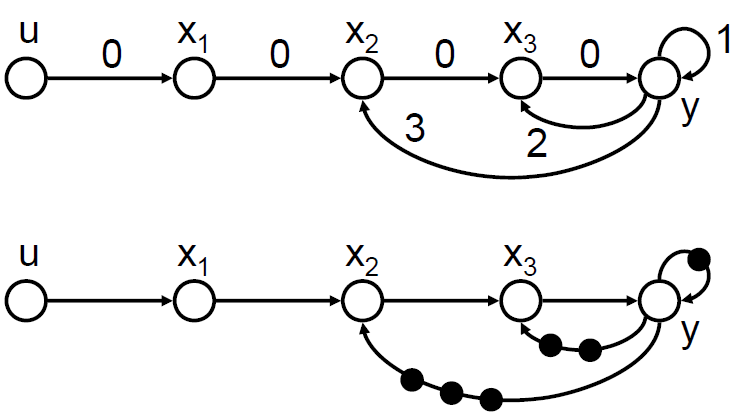
\includegraphics[scale=0.4]{img/11_iterativ_as_marked_graph.png}
	\caption{The iterative algorithm visualized as a marked graph.}
	\label{fig:iterative_as_marked_graph}
\end{figure}

Representation - signal flow graph

\begin{figure}[ht]
	\centering
  	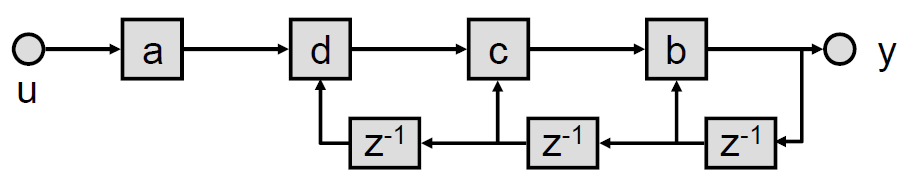
\includegraphics[scale=0.4]{img/11_iterativ_as_signal.png}
	\caption{The iterative algorithm visualized as a signal flow graph.}
	\label{fig:iterative_as_signal}
\end{figure}

Representation - Loop program


\begin{lstlisting}[mathescape][basicstyle=\tiny]
while(true)
{
	t1 = read(u);
	t5 = a*t1 + d*t2+c*t3+b*t4;
	t2  = t3;
	t3 = t4;
	t4 = t5;
	write(y, t5);
}
\end{lstlisting}


\begin{definition}[Iteration]
An iteration is the set of all operations necessary to compute all variables $x_i[l]$ for a fixed index $l$.
\end{definition}

\begin{definition}[Iteration interval]
The iteration interval $P$ is the time distance between two successive iterations of an integer algorithm.
\end{definition}

\begin{definition}[Throughput]
$1/P$ denotes the throughput of the implementation.
\end{definition}

\begin{definition}[Latency]
The latency $L$ is the maximal time distance between the starting and the finishing times of operations belonging to one iteration.
\end{definition}

\begin{definition}[Functional pipelining]
A pipelined implementation. Here exist time instances where the operations of different iterations $l$ are executed simultaneously.
\end{definition}

\begin{definition}[Loop folding]
In case of loop folding, starting and finishing times of an operation are in different physical iterations.
\end{definition}


Implementation principles
\begin{itemize}[noitemsep]
\item Simple possibility: the edges with $d_{ij} > 0$are removed from the extended sequence graph. The resulting simple sequence graph is implemented using standard methods.
\item Using functional pipelining: Successive iterations overlap and a higher throughput $1/P$ is obtained.
\end{itemize}

Solving the synthesis problem using  integer linear programming

\begin{itemize}[noitemsep]
\item Start with ILP formulation given for simple sequence graphs
\item Use the extended sequence graph with displacements $d_{ij}$
\item ASAP and ALAP scheduling for upper and lower bounds $h_i$ and $l_i$ use only edges with $d_{ij} = 0$
\item Suppose that a suitable iteration interval $P$ is choosen beforehand. If it is too small, no feasable solution to the ILP exists and P needs to be increased
\end{itemize}


Replacement of Equations
We can use the same equations, only replace 

\begin{itemize}[noitemsep]
\item (4) replaced by $\tau(v_j) - \tau(v_i) \geq w(v_i) - d_{ij} * P \qquad \forall (v_i, v_j ) \in E_S$
\item (5) is replaced by $ \sum_{\forall i : (v_i, v_k) \in E_R} \sum_{ p' = 0 }^{ w(v_i) -1} \sum_{\forall p : l_i \leq t - p' + p * P \leq h_i} x_{i, t-p'+p*P} \leq \alpha (v_k) \forall t: 1 \leq t \leq P, \forall v_k \in V_t$
\end{itemize}

\subsubsection{Dynamic Voltage Scaling}
We can transform the DVS problem into an integer linear program optimization: we can optimize the energy in case of dynamic voltage scaling.


Example of a set of tasks with dependency constraints:
\begin{itemize}[noitemsep]
\item We suppose that a task $v_i \in V_S$ can use one of the execution times $w_k(v_i) \forall k \in K$ and corresponding energy $e_k(v_i)$. There are $|K|$ different voltage levels.
\item We suppose that there are deadlines $d(v_i)$ for each operation $v_i$.
\item We suppose there are no resource constraints, can execute everything in parallel
\end{itemize}


\begin{enumerate}

\item minimize: $ \sum_{k \in K} \sum_{v_i \in V_S} y_{ik} * e_k(v_i)$ \\
	(sum up all individual energies of operations) \\
with subject to:
\item $y_{ik} \in \{ 0, 1\} \qquad \forall v_i \in V_S, k \in K$ \\
	(make decision variables $y_{ik}$ binary)
\item $\sum_{k \in K} y_{ik} = 1 \qquad \forall v_i \in V_S $ \\
	(guarantee that exactly one implementation $k \in K$ is choosen for each operation $v_i$)
\item $\tau(v_j) - \tau(v_i) \geq \sum_{k \in K} y_{ik} * w_k(v_i) \qquad \forall (v_i, v_j) \in E_S$ \\
	(implement the precedence constraints)
\item $\tau(v_i) + \sum_{k \in K} y_{ik} w_k(v_i) \leq d(v_i) \qquad \forall v_i \in V_S$ \\
	(guarantee deadlines)

\end{enumerate}



\cleardoublepage